% !TeX spellcheck = en_US
%===============================================================================
% $Id: ifacconf.tex 19 2011-10-27 09:32:13Z jpuente $
% Template for IFAC meeting papers
% Copyright (c) 2007-2008 International Federation of Automatic Control
%===============================================================================
\documentclass{ifacconf}

\usepackage{graphicx}      % include this line if your document contains figures
\usepackage{natbib}        % required for bibliography

\usepackage{fontspec}


\usepackage{amsmath}
\usepackage{amssymb}
\usepackage{color}
\usepackage{datetime}
\usepackage{placeins}
\usepackage{textcomp}
\usepackage{tikz}
\usepackage{pgfplots}
\pgfplotsset{compat=newest} 
\pgfplotsset{plot coordinates/math parser=false} 
\newlength\fheight
\newlength\fwidth

%===============================================================================

\graphicspath{
{../images/}{./images/}
}

% Custom commands
\newcommand{\mbf}[1]{\mathbf{#1}}
\newcommand{\idxFollower}{{\ensuremath{i} }}
\newcommand{\idxPredecessor}{{\ensuremath{i-1} }}
\newcommand{\idxSample}{{\ensuremath{k}}}
\newcommand{\idxAxis}{{\ensuremath{p}}}
\newcommand{\Francois}{\mbox{Fran\c{c}ois Defa$\ddot{\textrm{y}}$}}
\newcommand{\figheight}{4.8cm}
\newcommand{\figwidth}{6cm}

\newcommand{\Hinf}{\ensuremath{\textrm{H}_\infty} }
\newcommand{\Mu}{\ensuremath{\mu} \,}
\newcommand{\Htwo}{\ensuremath{\textrm{H}_2} }
\newcommand{\norm}[1]{\left\lVert#1\right\rVert}
\providecommand{\mbf}[1]{\mathbf{#1}}

% Rotation matrices
\newcommand{\Rbs}{{\ensuremath{\mbf{R_{b   s}}}}}
\newcommand{\Rbw}{{\ensuremath{\mbf{R_{b   w}}}}}
\newcommand{\Reb}{{\ensuremath{\mbf{R_{e  b}}}}}
\newcommand{\Reg}{{\ensuremath{\mbf{R_{e  g}}}}}
\newcommand{\Rbg}{{\ensuremath{\mbf{R_{b  g}}}}}
\newcommand{\Rgb}{{\ensuremath{\mbf{R_{g  b}}}}}
\newcommand{\Rbe}{{\ensuremath{\mbf{R^T_{e  b}}}}}
% Some useful symbols for the lazy:
\newcommand{\qbar}{\ensuremath{\bar{q}}}
\newcommand{\Matlabbrand}{Matlab\textsuperscript{\tiny{\textregistered}}}
\newcommand{\Simulinkbrand}{Simulink\textsuperscript{\tiny{\textregistered}}}

\begin{document}
\begin{frontmatter}

\title{An open benchmark for distributed formation flight control of Fixed-Wing Unmanned Aircraft Systems}

\author[First]{Jan Bolting}
\author[Second]{Martin Stolle}
\author[First]{Soheib Fergani}
\author[Second]{Jean-Marc Biannic}
\author[First]{\Francois}
 
\address[First]{Institut Supérieur de l'Aéronautique et de l'Espace (ISAE),
    31055 Toulouse, France (e-mail: jan.bolting@isae.fr, soheib.fergani@isae.fr, francois.defay@isae.fr)}
\address[Second]{Office National d'Études et de Recherches Aérospatiales (ONERA),
    31055 Toulouse, France (e-mail: jean-marc.biannic@onera.fr, martin.stolle@onera.fr)}
 
 
%\textcolor{red}{\Huge !!! DRAFT !!!\\ \normalsize \today \\ \currenttime}

% Abstract of not more than 250 words.
\begin{abstract}
The capability of autonomous formation flight has the potential to significantly enhance the utility and efficiency of small low-cost Unmanned Aerial Systems (UAS). Formations of small, inexpensive fixed-wing UAS allow for the sharing of remote sensing functionality, mission-level redundancy and range enhancements due to aerodynamic interactions widely exploited by migratory birds. This article presents a benchmark problem for scalable distributed flight control of formations of UAS with only local relative state information, one of the open problems in this field as of today. The benchmark is openly available and comprises a nonlinear six degrees of freedom dynamics model of an electric glider UAS.
In this article we furthermore introduce a nominal guidance frame that does not require state information of other UAS and point out a fundamental issue related to wake vortex tracking during formation maneuvers.
A set of LQ baseline controllers that are part of the benchmark is presented along with simulation results.
\end{abstract}
%
\begin{keyword}
UAS, Formation flight, benchmark
\end{keyword}

\end{frontmatter}
%===============================================================================

\section{Introduction}
Migratory birds routinely perform flights of several thousand kilometers. They do so using efficient formation patterns that allow them to benefit from the induced airflow generated by the birds upstream of them. Achievable energy savings of the order of 10 \% are reported in the literature, \cite{Weimerskirch2001}. For some time there have been efforts to imitate this behavior to enhance the range of aircraft. The NASA AFF program has demonstrated the feasibility of this approach for manned fighter aircraft in a 2-aircraft configuration. Maximum fuel flow reductions of 18 \% for the follower are reported, \cite{jake2003f}. \\
In terms of implementation effort, this strategy is a very attractive one, since no structural changes have to be made to the aircraft to gain considerable fuel savings (otherwise only achievable by considerable advancements in e.g. the fuel efficiency of the engines), only by adapting the flight control software and possibly adding sensors for relative localization. \\
In order to bring this capability to small unmanned aircraft, significant advances need to be made regarding relative guidance performance. Reported experimental results for 2-formations, \cite{Park2004}, and 3-formations, \cite{gu2006design}, feature relative guidance errors of the order of meters. However, both theoretical considerations \cite{Hummel1982} and flight experiments \cite{jake2003f} suggest that the UAS needs to stay in a window of wingtip-wingtip separations $(\Delta x \: \Delta y \: \Delta z)^T$ roughly specified by $\Delta y \in [-0.2b, -0.1b], \Delta z \in [-0.1b, 0]$ to benefit from significant energy savings. The longitudinal separation $\Delta x$ is less critical and can be several wingspans \cite{jake2003f}. For small UAS, the spanwidth $b$ is of the order of $1 \, m$, resulting in guidance error requirements of the order of $0.1 \, m$ laterally and vertically.
%
Testing autonomous formation flight control algorithms using inexpensive UAS also constitutes an interesting way for the commercial aviation industry to build confidence in and evaluate the safety implications new formation flight control systems before implementing them on manned aircraft.\\
%In this article we present a benchmark for distributed formation flight control of small UAS that will allow to evaluate competing control approaches on a unified test case.
In control, binary properties of a system such as stability or stability robustness - the system can either shown to be closed-loop stable over a given set of uncertainties or not - can usually be evaluated unambiguously for a given system. In contrast to that, control performance is tied to the problem that is used to evaluate a certain control approach. 
Benchmark problems play an essential role in every performance-driven field of research, as they allow to quantitatively compare different approaches. \\
As of today in the field of aircraft formation flight control there is no lack of contributions and promising approaches. However there appears to be a lack of reference problems to compare them and to make an informed judgment about their performance and implementability. This gap is it we are attempting to address with the presented benchmark. Inspired by existing benchmarks (\cite{biannic2015flare}) tailored to a specific challenging problem, e.g. Our modeling approach is focused on the current main issues of distributed formation control - mesh stability with minimum shared information and control performance that is compatible with the challenging demands of wake energy harvesting - and intentionally does not take into account secondary aspects such as sensor modeling and state estimation.\\
To be useful, a benchmark must be accessible to other researchers. Therefore, the proposed benchmark is complemented by an implementation as an openly accessible \Matlabbrand/\Simulinkbrand library. A set of LQ baseline controllers comes with the benchmark to provide a basic closed loop solution more advanced approaches can be compared to.
Furthermore, a cross-platform 3D visualization environment is part of the benchmark. \\
Numerous aircraft models \cite{Beard2012}, vortex simulation \cite{Dogan2008b,Saban2009} and trajectory planning techniques are available in the literature. Combining a specific set of these options into a simulation environment to evaluate a control technique constitutes a considerable, error-prone effort, and closed-loop results are not necessarily comparable due to the specificities of different modeling approaches or other subtleties such as simulation sampling times or assumed actuator model time constants. 
This work pulls together a number of contributions to provide a standard test case that addresses important challenges of distributed formation flight control as of today without requiring researchers to implement the simulation environment themselves.\\
The article is structured as follows: after elaborating on the role of information constraints on formation control in section \ref{sec:infoconstr}, the aircraft model and the simulation environment are presented in section \ref{sec:model}. Sections \ref{sec:trajectory} and \ref{sec:lqr} deal with the benchmark trajectory and baseline control laws, respectively. In section \ref{sec:simresults} first simulation results are presented and section \ref{sec:conclusio} provides some concluding remarks.
%
\section{Impact of information constraints}
\label{sec:infoconstr}
A variety of approaches for formation flight control have been proposed in the past. A focus has been formation scalability, i.e. the capability to add members to a formation without adapting control laws and without violating performance bounds. This is expressed by the requirement of mesh stability. In mesh stable formations, position errors stay locally confined and are not amplified while propagating through the formation.\\
As a general trend, the control problem becomes more challenging in inverse proportion to the available feedback information. Reduced feedback information is an attractive property, since less sensors and less inter-vehicle communications are necessary.
Centralized approaches, \cite{nageli2014environment}, pose no particular challenge, since standard control techniques can readily be applied, but require large amounts of inter-vehicle communication to obtain full state information. For mesh stable control with leader information linear techniques exist  \cite{shaw2007controller}.\\
The proposed benchmark addresses a more challenging scenario, distributed control with local state information, i.e. each member has only access to its own relative position and velocity w.r.t. to the preceding aircraft. 
There are fundamental results that linear interconnected systems with at least two integrators such as aircraft formations are always mesh unstable under local linear feedback (\cite{Pant2001}), ruling out linear control techniques.
Very few solutions based on nonlinear techniques such as Port-Hamiltonian systems, \cite{Knorn2014} and Sliding Mode control, \cite{galzi2006uav,Bolting2016}, have been proposed so far to tackle this problem and no experimental results are known to the authors. Furthermore, the existing approaches have been applied to very simplified models, basically point-mass approximations, neglecting a large part of the complex dynamics and constraints of a fixed-wing UAS. 
\section{Aircraft Model}
\label{sec:model}
\subsection{Aerodynamics}
There is an abundance of possibilities to model the aerodynamic coefficients of an aircraft, reaching from look-up tables to neural networks. Following the principle of minimum necessary complexity, here a classic, mostly linear in the states model of the aerodynamic force and moment coefficients has been adopted, \cite{Beard2012}
%
\begin{align}
\begin{split}
C_D =&\,C_{D_0} + \left(C_{L_0} + \frac{1}{\pi e \Lambda}C_{L_\alpha}\alpha\right)^2 + C_{D_{\delta_e}} + \frac{\bar{c}}{2V_a}C_{D_{q}}q
\label{eq:aerocoeffcd} \\
C_Y =&\,C_{Y_\beta}\beta + \frac{b}{2V_a} \left( C_{Y_p}p + C_{Y_r}r \right) + C_{Y_{\delta_a}}\delta_a + C_{Y_{\delta_r}}\delta_r\\
C_L =&\,C_{L_0} + C_{L_\alpha}\alpha +\frac{\bar{c}}{2V_a}C_{L_q}q +C_{L_{\delta_e}}\delta_e\\
C_l =&\,C_{l_{\beta}}\beta + \frac{b}{2V_a}\left(C_{l_{p}}p +C_{l_{r}}r\right) +C_{l_{\delta_a}}\delta_a +C_{l_{\delta_r}}\delta_r\\
C_m =&\,C_{m_0} + C_{m_\alpha}\alpha + \frac{\bar{c}}{2V_a}C_{m_q}q + C_{m_{\delta_e}}\delta_e\\
C_n =&\,C_{n_\beta}\beta + \frac{b}{2V_a} \left(C_{n_p}p + C_{n_r}r\right)+ C_{n_{\delta_a}} \! \delta_a+ C_{n_{\delta_r}}\!\delta_r
\end{split}
\end{align}
%
with the Oswald factor $e$ and the wing aspect ratio $\Lambda$. Estimates of the coefficients have been obtained with the software AVL from a 3D model of a small electric glider airplane, see \cite{StollePhD2016}.
\subsection{Kinematics}
Using \ref{eq:aerocoeffcd}, the aerodynamic forces and moments in the body frame are computed as
\begin{align}
\label{eq:coeff2realforcesandmoments}
%\begin{pmatrix}
%X \\ 
%Y \\
%Z 
%\end{pmatrix}
\mathbf{F}_a
&=
\Rbs
\bar{q}
S
\begin{pmatrix}
C_D \\ 
C_Y \\
C_L 
\end{pmatrix}
+
\begin{pmatrix}
T \\ 
0 \\
0 
\end{pmatrix}\\
% Moments.
%\begin{pmatrix}
%L \\ 
%M \\
%N 
%\end{pmatrix}
\mathbf{M}_a
&=
\Rbs
\begin{bmatrix}
\qbar S b & 0 & 0 \\
0 & \qbar S c & 0 \\
0& 0 & \qbar S b 
\end{bmatrix}
\begin{pmatrix}
C_l \\ 
C_m \\
C_n 
\end{pmatrix}
\end{align}
with $\Rbs$ the rotation matrix between stability frame and body frame, the vector of forces $\mathbf{F}_a$ and the vector of moments $\mathbf{M}_a$, assuming that the thrust vector is aligned with the body frame x axis and coincides with the center of gravity.
Translational accelerations in the body frame result to
\begin{align}
\label{eq:forces2accelerations}
\dot{\mathbf{v}}^b &= \frac{1}{m}\mathbf{F_a} 
- (\mathbf{\omega}^b \times \mathbf{v}^b) 
+
\Rbe
\mathbf{g}^e
\end{align}
where $\mathbf{v}^b$ is the translational velocity of the body frame w.r.t the inertial frame expressed in body frame axes, 
$\mathbf{\omega}^{b}$ is the angular velocity of the body frame w.r.t the inertial frame expressed in body frame axes and $\mathbf{g}^e$ is the gravity vector. The rotation rate of the earth can be neglected in this particular case due to the short duration of the considered UAS flight maneuvers.\\
Angular accelerations about body frame axes follow as
\begin{align}
\dot{\mathbf{\omega}}^b &= -\mathbf{J}^{-1} ({\mathbf{\omega}^b} 
\times 
(\mathbf{J} \,{\mathbf{\omega}^b}))
+ \mathbf{J}^{-1} 
\mathbf{M_a}
\end{align}
with the inertia tensor $\mathbf{J}$.
With these accelerations, standard integration techniques and transformations can be used to propagate angular and translational velocities and positions over time to compute the aircraft's full state, which is given by
\begin{align}
\mathbf{x} &= 
\begin{pmatrix}
\mathbf{p}^{e^T} \:
\mathbf{v}^{e^T} \:
\mathbf{q}^{T}_{eb} \:
\mathbf{\omega}^{b^T} \:
\end{pmatrix}^T 
\end{align}
with NED position $\mathbf{p}^e$, NED velocity $\mathbf{v}^e$, the attitude quaternion $\mathbf{q}_{eb}$ and the vector of rotation rate about body axes $\mathbf{\omega}^b$.
\subsubsection{Exogenous perturbations}
%
The aircraft dynamics are subject to exogenous disturbances due to atmospheric free air turbulence. These are taken into account as additional system inputs, extending the input vector to
%
\begin{align}
\mathbf{u} &= 
\begin{pmatrix}
\delta_{e} \:
\delta_{a} \:
\delta_{r} \:
\delta_{en} \:
\mathbf{v}_w^T \:
\mathbf{\omega}_w^T
\end{pmatrix}^T
\end{align}
\subsection{Actuators and Engine}
The control surface servo actuators have been identified in previous work, \cite{ameho2013pilotage}, as second order systems 
\begin{align}
\begin{pmatrix}
\dot{\delta}_i \\
\ddot{\delta}_i
\end{pmatrix}
=
\begin{bmatrix}
0 & 1 \\
-\omega_n^2 & -2 \zeta \omega_n 
\end{bmatrix}
\begin{pmatrix}
\delta_i \\
\dot{\delta}_i
\end{pmatrix}
+
\begin{bmatrix}
0\\
\omega_n
\end{bmatrix}
\delta_{i, c}
\end{align}
where $\omega_n=62.8 \, s^{-1}$ and $\zeta=0.8$.
This model is augmented by adding realistic saturations on deflection and deflection rate
%
\begin{align}
|\delta_i| \in [-\frac{\pi}{4}, \; \frac{\pi}{4}]\, rad, |\dot{\delta}_i| \in [-5.8, 5.8] \frac{rad}{s}
\end{align}
The engine is modeled as first order system
%
\begin{align}
\dot{\delta}_{en}
=
\tau_{en}^{-1}
(
\delta_{en, c}
- \delta_{en}
)
\end{align}
%
where $\tau_{en} = 0.27^{-1}s^{-1}$. The thrust $T$ is then computed using a simple model based on momentum theory (\cite{Beard2012}) as
%
\begin{align}
T = \frac{\rho}{2}
S_{en}
C_{en} 
(
(k_{en}\delta_{en})^2
-V_a^2
)
\end{align}
with the propeller disc surface $S_{en}$, the thrust constant $C_{en}$, the engine constant $k_{en}$ and the airspeed $V_a$.
%
%\subsection{Vortex Model}
%A variety of approaches has been proposed to simulate the effects of trailing vortices on the following UAS, mostly based on modified Horseshoe Vortex models (HVM) \cite{Hummel1982} or Vortex Lattice methods (VLM) \cite{Saban2009}. For the purpose of this work, a model based on a HVM with modified core model \cite{dogan2005modeling} is used. It is reported to provide predictions that are in good agreement with both VLM models and wind tunnel measurements. By using an averaging scheme, induced velocities and angular rates are generated in function of the inter-UAS separation vectors.
%
\subsection{Wind}
The wind is assumed to be composed of a constant ambient part and a time-varying stochastic part, inducing velocities
\begin{align}
\mathbf{v}_w(t) = \mathbf{v}_{w,a} + \mathbf{v}_{w,s}(t)
\end{align}
and induced angular rates
$\mathbf{\omega}_w(t)$. 
Wind time series are generated according to the Dryden turbulence spectrum (\cite{standardflying}) as implemented by the \Matlabbrand / \Simulinkbrand Aerospace Blockset\textsuperscript{\texttrademark}.
\section{Benchmark Trajectory}
\label{sec:trajectory}
The benchmark includes a 3D trajectory composed of $\mathrm{C}_2$-continuous cubic Bézier splines, based on the work presented by \cite{Yang2008}. The trajectory features a linear part to evaluate cruise flight performance, followed by an approximately helical part to evaluate climb and turn maneuvers. See \cite{looye2011helical} for the compelling properties of helical trajectories for the evaluation of automatic flight control laws.
%
\begin{figure}
\centering
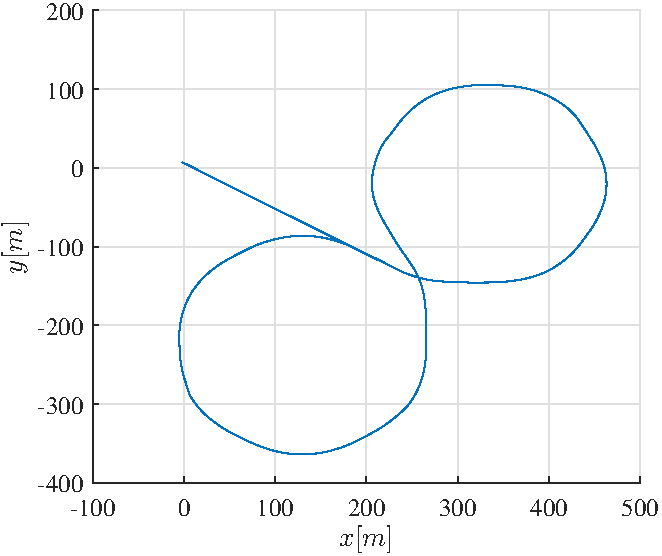
\includegraphics[width=.6\columnwidth]{trajectory.pdf}
\caption{Top view of benchmark trajectory}
\end{figure}
%
%\begin{figure}
%\centering
%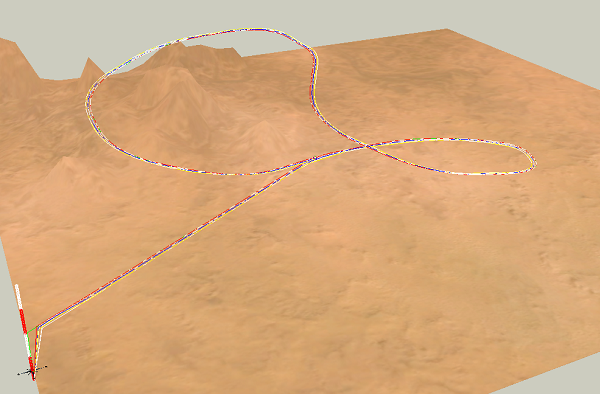
\includegraphics[width=.8\columnwidth]{UAV3D_helix-lowres}
%\caption{Isoview of benchmark trajectory in UAV3D}
%\end{figure}
%
\section{LQ baseline control laws}
\label{sec:lqr}
To provide a standard to compare new control approaches, a set of baseline LQ control laws is provided as part of the benchmark. For controller synthesis, the respective subsystems are extracted from the full linear model that results from linearizing the nonlinear aircraft model at cruise flight trim conditions. The structure of the control laws is based on the usual assumptions of weak coupling between lateral and longitudinal dynamics and timescale separation of attitude dynamics and translational dynamics.\\
The synthesis procedure is the same for all four subsystems. It is shortly recalled here, and the specific design systems for every controller are given in the respective subsections. 

\noindent
The time-invariant linear quadratic regulator (LQR) minimizes a quadratic integral performance index
\begin{align}
J = \int_{t0}^{\infty}(
\mathbf{x}(t)^T 
\mathbf{Q}
\mathbf{x}(t)
+
\mathbf{u}(t)^T 
\mathbf{R}
\mathbf{u}(t)
)
dt
\end{align}
for a given linear system
\begin{align}
\dot{\mathbf{x}}(t)
=
\mathbf{A}
\mathbf{x}(t)
+
\mathbf{B}
\mathbf{u}(t)
\end{align}
where $\mathbf{x} \in \mathbb{R}^n$ and $\mathbf{u} \in \mathbb{R}^m$ are the state and input vectors respectively and $\mathbf{Q} \in \mathbb{R}^{n\times n}$ and $\mathbf{R} \in \mathbb{R}^{m\times m}$ are positive definite design matrices.
To track a given reference state $\mbf{x}_c$, the tracking error dynamics are derived (dropping in the following the explicit dependence on time) as
\begin{align}
\dot{\mathbf{x}}_e
&=
\dot{\mbf{x}}
-
\dot{\mathbf{x}}_c \\
{}
&=
\mathbf{A}
\mathbf{x}
+
\mathbf{B}
\mathbf{u}
-
\dot{\mathbf{x}}_c 
\end{align}
The reference state is either constant, as in the static relative position tracking case, or unknown, since the reference state (e.g. the commanded bank angle) is generated by the outer loop controller. Its derivative is thus treated as unknown disturbance and set to zero for controller design, leading to the state error dynamics
that are identical with the state dynamics. 
\begin{align}
\dot{\mathbf{x}}_e
&=
\mathbf{A}
\mathbf{x}
+
\mathbf{B}
\mbf{u}
\end{align}
Tracking is thus approached by a simple change of state coordinates
\begin{align}
\dot{\mbf{x}}_e
&=
{\mbf{x}}
-
{\mbf{x}}_c 
\label{eq:errorss}
\end{align}
To cope with steady state tracking errors, integral action is added by augmenting the system (\ref{eq:errorss}) with integral states
\begin{align}
\begin{pmatrix}
\dot{\mbf{x}}_e \\
\dot{\mbf{x}}_i
\end{pmatrix}
&=
\begin{bmatrix}
\mbf{A} & \mbf{0} \\
\mbf{G} & \mbf{0}
\end{bmatrix}
\begin{pmatrix}
\mbf{x}_e \\
\mbf{x}_i
\end{pmatrix}
+
\begin{bmatrix}
\mbf{B} \\
\mbf{0}
\end{bmatrix}
\mbf{u}
\label{eq:integerrorss}
\end{align}
where $G$ is a sparse matrix defining the states that are selected for integral action. As is common practice, wind disturbances and actuator and engine dynamics are neglected for the LQR design systems. 
%A linear model including models of actuators and engine is used for fast evaluation of candidate controllers during controller tuning.
\subsection{Coordinate frames}
The system to be controlled is a formation of $n$ UAS flying in an arbitrary pattern. In the literature, a variety of guidance frames has been proposed, ranging from a planar frame aligned with the follower's velocity (\cite{gu2006design}) to the predecessor's body frame (\cite{schumacher2000adaptive}).
The primary objective of tight formation flight is to keep each UAS at the position of maximum efficiency in the wake of its predecessor.
Being induced by the aerodynamic flow, the wake vortices are approximately aligned with the predecessor's wind frame, neglecting trajectory curvature. 
For maximum energy savings, the follower thus needs to keep its relative position constant in this frame. Since small UAS typically are not equipped with sensors for angle of attack and side slip angle, a local guidance frame (index $g$) is introduced as an approximation. Its x axis unit vector $\mbf{u}_{x,g}$ is aligned with each predecessor's NED velocity vector. Its y axis should be aligned with the y axis of the predecessor's body frame, since the central axis of the vortices lies somewhere on the predecessor's wing.
To avoid having to communicate the NED speed and attitude of each UAS to its follower, the nominal speed and acceleration vector of each UAS on the current formation trajectory is used to derive a nominal guidance frame.
These two vectors are computed sequentially for each UAS, since the attitude of each nominal local guidance frame defines the nominal NED position of the next one.
For two subsequent UAS, predecessor $p$ and follower $f$, the nominal NED speed of $f$ is computed as
\begin{align}
\mbf{v}_f^e &= \mbf{v}_p^e + \mbf{\omega}_p^e \times \Delta \mbf{p}_f^e 
\end{align}
with the commanded separation vector $\Delta \mbf{p}_f^e$ and the rotation rate vector $\mbf{\omega}_p^e$ corresponding to the leader's trajectory curvature. Nominal acceleration of $f$ is given by
\begin{align}
\dot{\mbf{v}}_f^e &= \dot{\mbf{v}}_p^e + \mbf{\omega}_p^e \times (\mbf{\omega}_p^e \times \Delta \mbf{p}^e_f)
\end{align}
and the instantaneous rotation rate $\mbf{\omega}_p^e$ of the guidance frame due to trajectory curvature by
\begin{align}
|\mbf{\omega}_p^e| &= {|{\mbf{v}_g^e}|}^{-1}{|\dot{\mbf{v}_g^e}|}\\
\mbf{\omega}_p^e &= 
|\mbf{\omega}_p^e| 
({\dot{\mbf{v}_p^e} \times \mbf{v}_p^e})({|\dot{\mbf{v}_p^e} \times \mbf{v}_p^e|})^{-1}
\end{align}
The x axis unit vector of the local guidance frame results then to
\begin{align}
\mbf{u}_{x,g} = |\mbf{v}_p^e|^{-1}\mbf{v}_p^e
\end{align}
The orientation of the z axis unit vector $\mbf{u}_{z,g}$ is derived from the simplifying assumption that gravitational acceleration and centrifugal forces due to trajectory curvature are compensated for by the thrust and drag along $\mbf{u}_{x,g}$ and by the aerodynamic lift in a plane normal to $\mbf{u}_{x,g}$. Further assuming that the aerodynamic lift $Z$ lies in the x-z plane of the body frames, first the total centrifugal and gravitational acceleration acting on $p$ is computed as
\begin{align}
\mbf{a}_{t} = |\mbf{\omega}^e_{p}|^2 \mbf{r} + \mbf{g}^e
\end{align}
The z unit vector $\mbf{u}_z$ is then computed by projecting and normalizing the total acceleration on the z-y plane of the g frame
\begin{align}
\mbf{a}_{t,zy} = \mbf{a}_t - \frac{\mbf{a}_t \cdot \mbf{u}_{x,g}}{\mbf{u}_{x,g} \cdot \mbf{u}_{x,g}} \cdot \mbf{u}_{x,g} \\
\mbf{u}_{z,g} = |\mbf{a}_{t,zy}|^{-1}\mbf{a}_{t,zy}
\end{align}
and $\mbf{u}_{y,g}$ completes a right-handed Cartesian coordinate frame
\begin{align}
\mbf{u}_{y,g} = \mbf{u}_{z,g} \times \mbf{u}_{x,g}
\end{align}
leading to the corresponding rotation matrix
\begin{align}
\Reg 
=
\begin{bmatrix}
\mbf{u}_{x,g} & 
\mbf{u}_{y,g} &
\mbf{u}_{z,g}
\end{bmatrix}
\end{align}
%
%Baaam: tracking the vortex during maneuvers makes trajectory disturbances formation-size dependent, independently of the used controllers.
%The system to be controlled is a formation of $n$ UAS flying in an arbitrary pattern. The right choice of reference frames can significantly facilitate control design. To give one example, when performing navigation in the predecessor's body frame, variations in the predecessor's attitude will couple into follower's position control loops, increasing control action. What is more, the effect increases with inter-vehicle separation, leading to high control demands during rendezvous. To avoid such disadvantages, the motion of the reference frame with respect to the inertial frame should be within the control bandwidth of the position controller. A suitable frame is a local Cartesian frame whose x axis is aligned with the follower's inertial speed projected on the horizontal plane, and whose z axis is aligned with the NED frame's z axis, the \textbf{Follower Speed Frame} (FS). Its origin coincides with the follower's body frame. The follower's wind frame would be preferable, but requires on-line wind estimation or flow sensors that usually are not available for small UAS.
%To dispose of a common reference frame for multiple members of the formation, the \textbf{Leader Speed Frame} (LS) is defined. Its x axis is aligned with the formation leader's NED speed projected on the horizontal plane, its z axis is aligned with the NED frame's z axis, and its y axis completes a right-handed Cartesian coordinate system.
\subsection{Predecessor tracking}
\subsubsection{Longitudinal}
The control inputs of the longitudinal position control loop are the commanded pitch angle $\Theta_c$ and the engine command $\delta_{en,c}$. In the absence of external disturbances it regulates the relative position and velocity errors asymptotically to zero. Using $\Theta_c$ as control input instead of the angle of attack $\alpha$, which is more directly related to aerodynamic lift, is imposed by the usual absence of AoA sensors on board of small UAS. To obtain a good approximation of $\alpha$, the pitch angle w.r.t to the local guidance frame is used. The design system is given by
%
\begin{align}
\begin{pmatrix}
\Delta \dot{p}_x \\
\Delta \dot{p}_z \\
\Delta \dot{v}_x \\
\Delta \dot{v}_z \\
\Delta \dot{p}_{x,int} \\
\Delta \dot{p}_{z,int} 
\end{pmatrix}
=
\begin{bmatrix}
\mbf{
A
}_{lon, pos} 
& 
\mbf{0} 
\\
\begin{bmatrix}
\mbf{I}_2 & \mbf{0}_{2}
\end{bmatrix}
& 
\mbf{0}
\end{bmatrix}
\begin{pmatrix}
\Delta {p}_x \\
\Delta {p}_z \\
\Delta {v}_x \\
\Delta {v}_z \\
\Delta {p}_{x,int} \\
\Delta {p}_{z,int} 
\end{pmatrix}
+
\mbf{
B
}_{lon, pos}
\begin{pmatrix}
\delta_{en} \\
\Theta_c
\end{pmatrix}
\end{align}
\subsubsection{Lateral}
The lateral control strategy is derived from the simplified system
\begin{alignat}{3}
{} &&n_y &= \frac{Z}{m g} \sin(\Phi) \\
{} &&Z   &\approx m g \\
\Rightarrow &&n_y &\approx \sin^{-1}(\Phi) \label{eq:ny2phi}
\end{alignat}
%
thus lateral load factors in the local guidance frame are generated by inclining the lift vector via the local bank angle $\Phi$. The resulting LQR design system is given by
%
\begin{align}
\begin{pmatrix}
\Delta \dot{p}_y \\
\Delta \dot{v}_y \\
\Delta \dot{p}_{y,int} 
\end{pmatrix}
=
\begin{bmatrix}
\mbf{
A
}_{lat, pos} 
& 
0
\\
\begin{bmatrix}
1 & 0
\end{bmatrix}
& 
0
\end{bmatrix}
\begin{pmatrix}
\Delta {p}_y \\
\Delta {v}_y \\
\Delta {p}_{y,int} 
\end{pmatrix}
+
\mbf{
B
}_{lat, pos}
\begin{pmatrix}
n_{y,c}
\end{pmatrix}
\end{align}
and the commanded bank angle in the local guidance frame is computed using  (\ref{eq:ny2phi}).
\subsection{Attitude tracking}
The inner loops consist of separate pitch angle and bank angle tracking laws. Both angles are not the usual Euler angles w.r.t. to the NED frame but are defined as the rotation angles needed to rotate the body frame into the local guidance frame. That being said, the resulting commanded attitude rotation matrix w.r.t. to the NED frame is composed as
\begin{align}
\Reb_{,c} 
= 
\Reg \: \Rgb_{,c} (\Phi_c, \Theta_c)
\end{align}
where
\begin{align}
\Rgb_{,c} (\Phi_c, \Theta_c)
= 
\begin{bmatrix}
\cos \Phi_c &  \sin \Phi_c \cos \Theta_c & \sin \Phi_c \cos \Theta_c \\
-\sin \Phi_c& \cos \Phi_c \cos \Theta_c  & \cos \Theta_c \sin  \Theta_c \\
0 & -\sin \Theta_c & \cos \Phi_c
\end{bmatrix}
\end{align}
Note that the local heading angle is not actively controlled and as such is set to zero.
%
\subsubsection{Longitudinal}
The pitch attitude design system is given by
\begin{align}
\begin{pmatrix}
\Delta \dot{\Theta} \\
\dot{q} \\
\Delta \dot{\Theta}_{int} 
\end{pmatrix}
=
\begin{bmatrix}
\mbf{
A
}_{lon, att} 
& 
0
\\
\begin{bmatrix}
1 & 0
\end{bmatrix}
& 
0
\end{bmatrix}
\begin{pmatrix}
\Delta {\Theta} \\
{q} \\
\Delta {\Theta}_{int} 
\end{pmatrix}
+
\mbf{
B
}_{lon, att}
\begin{pmatrix}
\delta_{e}
\end{pmatrix}
\end{align}
\subsubsection{Lateral}
The lateral attitude law is driven by two requirements: tracking a commanded local bank angle and adding damping to the weakly damped dutch roll mode. The second one is achieved by adding the yaw rate $r$ to the state vector of the design system and choosing an appropriate weight in the LQR synthesis matrix $\mbf{Q}$. The design system is thus:
\begin{align}
\begin{pmatrix}
\Delta \dot{\Phi} \\
\dot{p} \\
\dot{r} \\
\Delta \dot{\Phi}_{int} 
\end{pmatrix}
=
\begin{bmatrix}
\mbf{
A
}_{lat, att} 
& 
0
\\
\begin{bmatrix}
1 & 0 & 0
\end{bmatrix}
& 
0
\end{bmatrix}
\begin{pmatrix}
\Delta {\Phi} \\
{p} \\
{r} \\
\Delta {\Phi}_{int} 
\end{pmatrix}
+
\mbf{
B
}_{lat, att}
\begin{pmatrix}
\delta_a \\
\delta_r \\
\end{pmatrix}
\end{align}
\section{Simulation results}
\label{sec:simresults}
Flight on the benchmark trajectory has been simulated for a formation of three UAS both in calm air and under turbulent wind with $\mbf{v}_{w,a} = (-3 \; -3 \; 0)^T \, \frac{m}{s}$ i.e. about $28 \, \%$ of the nominal airspeed of $15 \, \frac{m}{s}$. The separation vectors have been selected as $\Delta \mbf{p}_i (-b \: b \: 0)^T$ for $i=1...3$.
\subsection{Visualization}
A lightweight visualization environment based on the Java jmonkey game engine (see \cite{jmonkeyengine}) has been developed to display the attitude and positions of multiple UAS in a synthetic 3D environment. 
It has proven to enhance productivity while developing and debugging guidance laws. 
It is interfaced with the Simulink dynamics simulation via a UDP (User Datagram Protocol) network link. Visuals have to be updated only at a moderate rate of about 30 Hz for human perception, thus sending UDP packets adds a small simulation time overhead. The tool is open software and currently provides several generic UAS 3D models as well as the possibility to display wake vortices.
%\begin{figure}
%\centering
%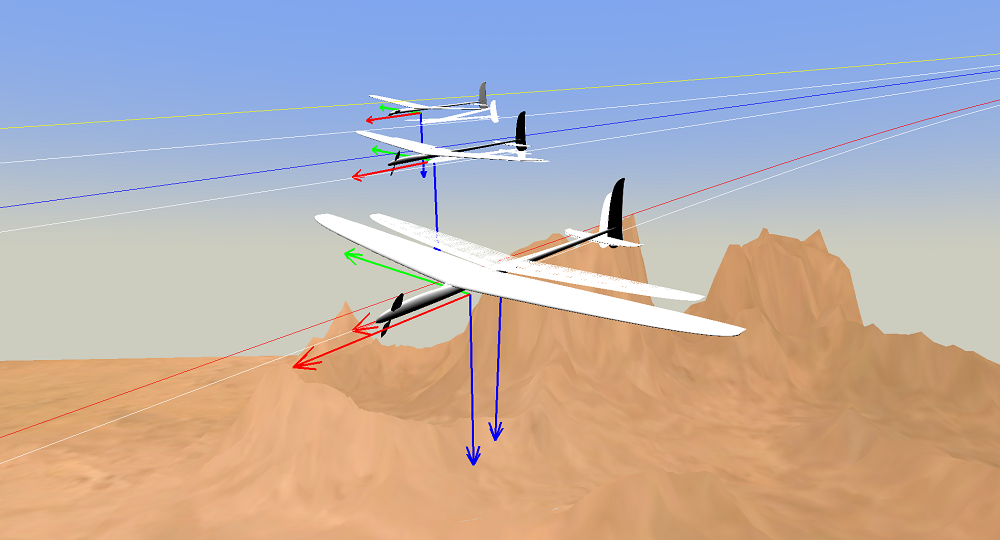
\includegraphics[width=.8\columnwidth]{UAV3D_N=3-lowres}
%\caption{N=3 formation in UAV3D}
%\end{figure}
\subsection{Calm atmosphere}
\label{sec:simresults_calm}
Position errors in the local guidance frames along with the longitudinal control inputs under calm air conditions are shown in fig. \ref{fig:combinedcalmair}. Simulating the benchmark formation in calm air clearly reveals two deficiencies of the baseline controllers. The first is their expected mesh instability. The second one is related to the selection of guidance frames, see section \ref{sec:lqr}. Since the local guidance frames have been selected to track the predecessor's wake vortices, changes of trajectory curvature create perturbations w.r.t. the NED frame that are dependent on the separation vectors and vehicle index. This leads - with linear controllers - to position errors that grow with the vehicle index.  Tracking the vortex during maneuvers is therefore not a scalable guidance strategy. This constitutes an open problem.
%
\begin{figure}
\centering
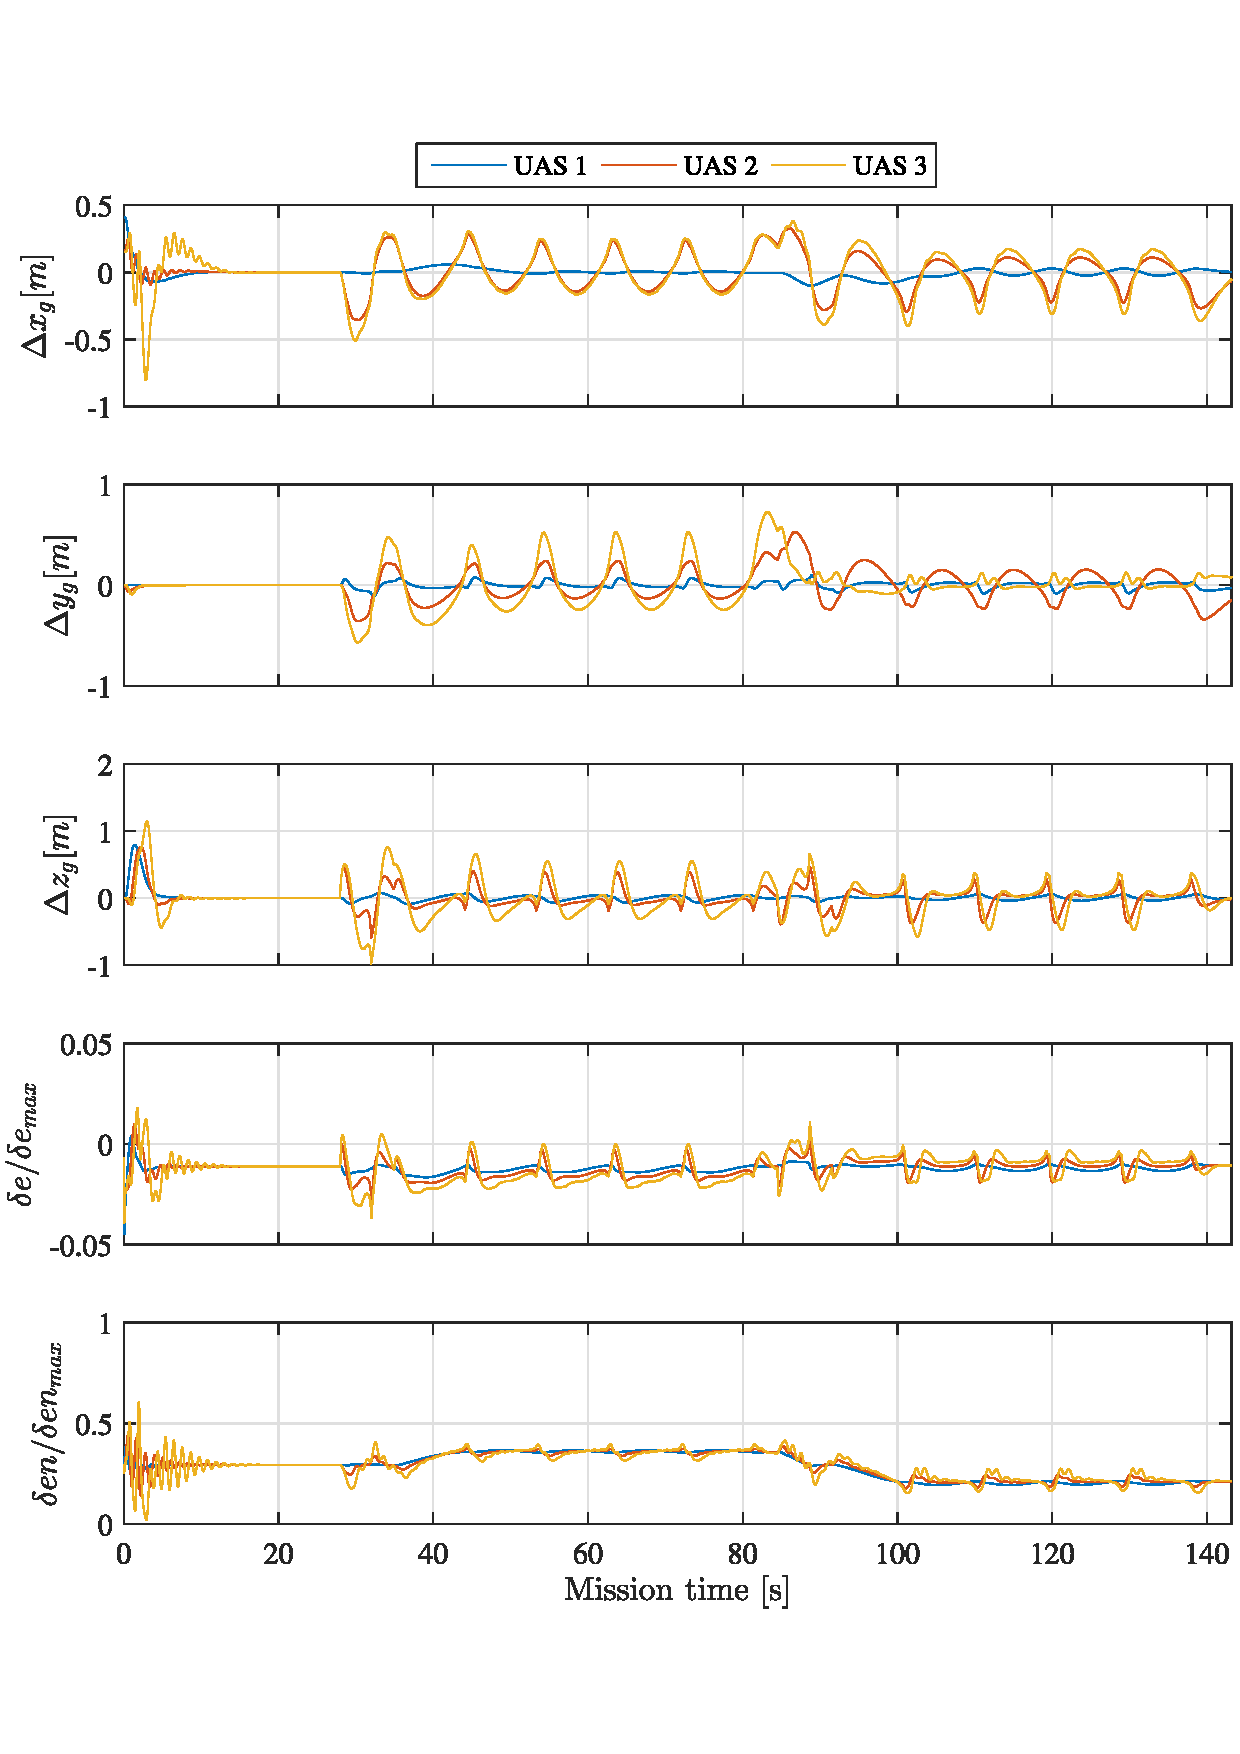
\includegraphics[width=.8\columnwidth, height=.75\columnwidth]{combined-calmair-lowres.pdf}
\caption{Position errors in \textit{g} frame and longitudinal control inputs for calm atmosphere}
\label{fig:combinedcalmair}
\end{figure}
%
\subsection{Turbulent atmosphere}
Position errors in the local guidance frames along with the longitudinal control inputs under wind and turbulence are shown in fig. \ref{fig:combinedcalmair}. Position errors are considerably larger during the initial cruise flight phase. On the helical part of the trajectory, perturbations due to reference frame perturbations dominate. The helical trajectory clearly reveals another shortcoming of the baseline control strategy. As the formation descends and the changing trajectory heading leads to tailwind, the engine inputs saturate as the longitudinal position controller attempts to maintain constant ground speed. It seems therefore advisable to add some kind of wind estimation scheme into the guidance strategy to maintain constant airspeed.
\begin{figure}
\centering
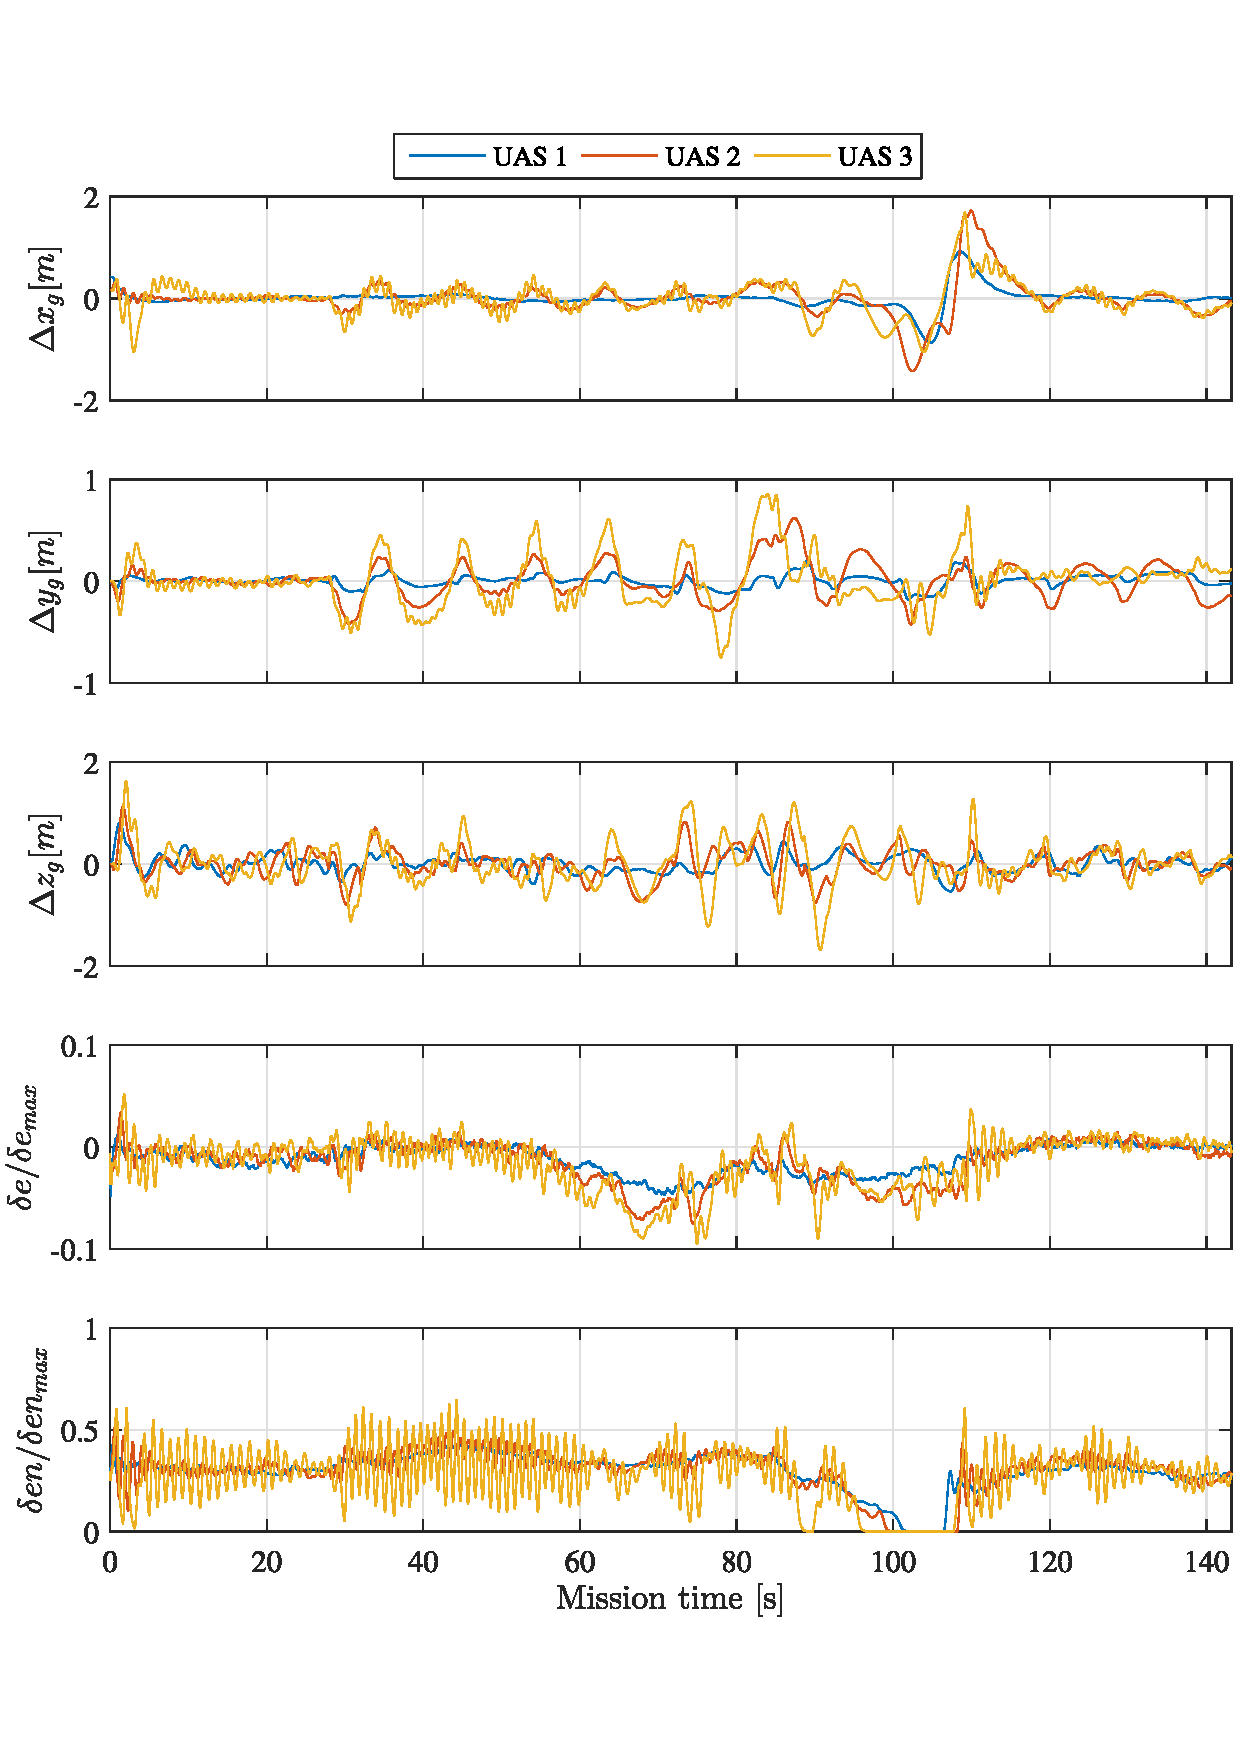
\includegraphics[width=.75\columnwidth, height=.75\columnwidth]{combined-turbulentair-lowres.pdf}
\caption{Position errors in \textit{g} frame and longitudinal control inputs for turbulent atmosphere}
\end{figure}
%
\section{Conclusion}
\label{sec:conclusio}
A new benchmark for distributed formation flight control for small UAS has been presented, along with simulation results for a set of baseline controllers. The results confirm their expected mesh instability as well as the ability of the chosen reference trajectory to reveal this and various other deficiencies of the baseline guidance strategy. These deficiencies provide a starting point for future improvements. It is demonstrated that tracking the predecessor's wake vortex during maneuvers is not a scalable guidance strategy. \\
We invite other researchers working in this domain to adopt this benchmark to evaluate new promising control and guidance approaches such as \cite{padhi2014formation} and to contribute to it e.g. by proposing and implementing new benchmark trajectories or by adding to the documentation. The benchmark and the tools it is built on are version controlled for guaranteed comparability and openly available, \cite{UAV3D,ffb}. The implementation depends on a number of \Matlabbrand/\Simulinkbrand toolboxes and blocksets. To reduce this threshold, we are currently evaluating the possibility of a hosted benchmark that is accessible via the Internet.
%
\bibliography{bibliography/bibliographyPhD}      
\end{document}
